% relatorio do t1 de computacao paralela - paralelizacao de path tracer smallpt
% formato conforme enunciado corrigido: A4, margem >= 1.5cm, fonte 10-11,
% espacamento simples, ate 2 paginas, coluna dupla (opcional).
\documentclass[10pt,a4paper]{article}

\usepackage[utf8]{inputenc}
\usepackage[T1]{fontenc}
\usepackage[portuguese]{babel}
\usepackage[margin=1.5cm]{geometry}
\usepackage{multicol}
\usepackage{graphicx}
\usepackage{booktabs}
\usepackage{caption}
\usepackage{microtype}
\usepackage{amsmath}
\usepackage{parskip}
\usepackage{hyperref}
\hypersetup{colorlinks=true, linkcolor=black, urlcolor=blue}

\setlength{\columnsep}{0.6cm}
\setlength{\parskip}{2pt}
\setlength{\parindent}{0pt}
\captionsetup{font=small,labelfont=bf,skip=2pt}

\pagestyle{empty}

\begin{document}

% cabecalho reduzido: sem capa. identificacao do grupo e do trabalho.
\begin{center}
  {\large\bfseries T1 -- Paralelizacao de uma aplicacao com OpenMP} \\[2pt]
  {\small Computacao Paralela -- Unidade 03 \quad|\quad Aluno: Bernardo Klein Heitz} \\[1pt]
  {\footnotesize Codigo entregue em .zip junto deste PDF.}
\end{center}

\begin{multicols}{2}

\section*{1. Introducao}
Paralelizamos com OpenMP um \emph{path tracer} do estilo \texttt{smallpt} de
Kevin Beason, reescrito em C. O programa renderiza uma Cornell Box com nove
esferas (paredes difusas, uma esfera especular e uma refrativa) usando
Monte Carlo com amostragem estratificada 2$\times$2 por pixel e roleta russa a
partir da profundidade 5. A escolha atende os quatro criterios do enunciado:
tempo sequencial na janela de 30 a 60\,s, um laco externo independente por
linha, complexidade nao trivial (materiais e reflexoes) e entrada
parametrizavel por \texttt{-w W -h H -s SPP}.

\section*{2. Ambiente e metodologia}
CPU: AMD Ryzen 5 3600 (6 nucleos fisicos, 12 processadores logicos,
3.6\,GHz base), cache L3 de 32\,MB, 32\,GB de RAM DDR4. SO: Ubuntu 22.04
em WSL2 sobre Windows 10. Compilador: \texttt{gcc 11.4.0}. Flags identicas
nas duas versoes: \texttt{-O3 -march=native -ffast-math -std=c11}; a
versao paralela acrescenta apenas \texttt{-fopenmp}.
\texttt{omp\_get\_num\_procs()} devolve 12, igual a \texttt{nproc}.
\textbf{Regiao medida:} \texttt{omp\_get\_wtime()} envolve a fase
computacional completa -- setup da camera, alocacao do buffer, laco de
renderizacao e checksum. A escrita PPM e o print do CSV ficam fora; os
mesmos limites valem nas duas versoes. O tempo isolado do trecho
paralelizado e reportado em \texttt{time\_par\_s} como medida complementar.
\textbf{Entrada de referencia:} \texttt{w=800 h=600 spp=32}, com
$T_1 \approx 54$\,s. \textbf{Protocolo:} 10 execucoes por configuracao,
maquina ociosa; tabelas com mediana, min e max. \textbf{Threads:}
\texttt{OMP\_NUM\_THREADS}. \textbf{Validacao:} checksum RGB identico entre
1 e 12 threads e entre todas as politicas de escalonamento.

\section*{3. Perfil e teto de Amdahl}
O \texttt{gprof} foi levantado na mesma entrada e na mesma fase do
speed-up (binario \texttt{-O2 -fno-inline -pg}). \texttt{radiance} e
suas chamadas somam 98{,}2\% do tempo; \texttt{main} fica com 1{,}75\%.
A fracao paralelizavel e $f \approx 0{,}982$. Os limites de Amdahl sao
$S_{\max}(6) \approx 5{,}51$, $S_{\max}(12) \approx 10{,}00$ e o limite
assintotico $S_{\infty}=1/(1-f)\approx 55{,}6$. No binario \texttt{-O3},
\texttt{time\_par\_s}/\texttt{time\_s} da versao sequencial e $0{,}99998$:
a parcela sequencial da fase medida e desprezivel. A saturacao da
Secao~6 fica abaixo de $S_{\max}(12)$, logo nao se deve a essa fracao.

\section*{4. Modelagem e diretivas}
A unidade de trabalho e uma linha da imagem. O laco em \texttt{y} tem
600 iteracoes; cada uma escreve numa faixa disjunta de \texttt{c}, o que
dispensa \texttt{atomic}, \texttt{critical} e \texttt{reduction} no caminho
quente. O gerador xorshift64 e local ao corpo do laco e recebe semente
derivada da linha, o que torna o checksum independente do numero de threads.

Os pragmas essenciais estao em \texttt{src/smallpt.c:319--331}:
\begin{quote}\small\ttfamily
\#pragma omp parallel default(none) \\
\quad shared(a, c, cam\_o, cam\_d, cx, cy, stat, threads\_used) \\
\{ \\
\quad \#pragma omp for schedule(runtime) nowait \\
\quad for (int y = 0; y < a.h; ++y) \{ ... \} \\
\}
\end{quote}
O \texttt{default(none)} obriga listar o escopo. \texttt{c} tem escrita
disjunta; \texttt{stat} e indexado por \texttt{omp\_get\_thread\_num()}
com padding de 64\,B. \texttt{schedule(runtime)} troca a politica por
\texttt{OMP\_SCHEDULE}; \texttt{nowait} faz o perfil por thread refletir
o trabalho real, nao a barreira.

\section*{5. Balanceamento medido}
Sete politicas em 12 threads, 10 execucoes cada (Tabela\,\ref{tab:sched}).
\texttt{dynamic,4} teve a menor mediana (7{,}16\,s) e a menor dispersao
(7{,}01 a 7{,}35\,s). \texttt{static} sem chunk ficou em ultimo
(9{,}56\,s), com amostras de 7{,}57 a 11{,}78\,s, embora o perfil
interno com \texttt{nowait} mostre desbalanceamento inferior a 1\%.
A variancia por profundidade de raio nao explica esse gap: em WSL2 uma
thread preemptada no \texttt{static} trava o programa, enquanto
\texttt{dynamic,4} redistribui blocos. Adotamos \texttt{dynamic,4} por
essa medicao.

\section*{6. Analise dos resultados}
A Figura\,\ref{fig:speedup} e a Tabela\,\ref{tab:strong} mostram a
escalabilidade forte. Ate 6 threads o speed-up acompanha Amdahl
(4{,}93 medidos contra 5{,}51, eficiencia 82{,}2\%). No ponto em que o
SMT entra (linha vertical em 6 threads) a curva se dobra: de 6 para 8 o
ganho vai a 6{,}14 (+25\%) e a eficiencia cai a 76{,}8\%; de 10 para 12
o ganho adicional e 1{,}8\% e a eficiencia cai a 62{,}0\%. O
\texttt{smallpt} e compute-bound em \texttt{double}; duas threads no
mesmo nucleo competem pelas unidades de ponto flutuante. O speed-up
7{,}44 em 12 threads fica abaixo de $S_{\max}(12)\approx 10$, portanto
a saturacao e SMT (e preempcao do WSL2), nao a fracao sequencial.

\begin{center}
  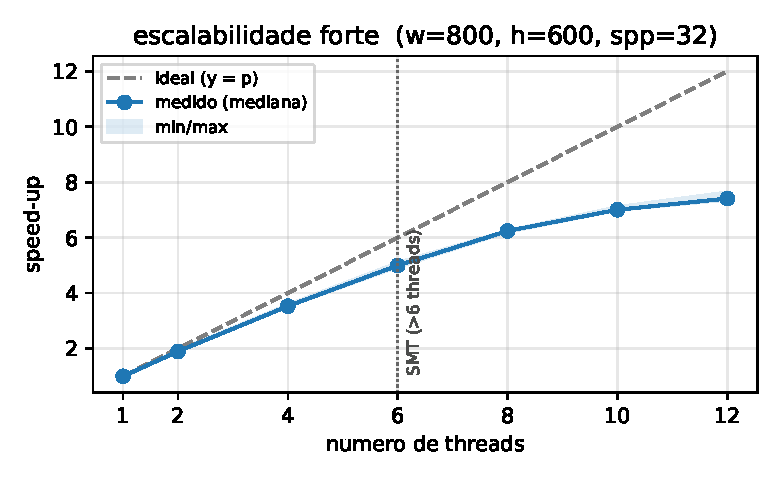
\includegraphics[width=\linewidth]{../results/speedup.pdf}
  \captionof{figure}{Speed-up medido (mediana de 10 execucoes) contra a
    reta ideal $y=p$. A faixa clara e o intervalo min--max. A linha
    vertical em 6 threads marca o ponto em que o SMT passa a atuar.}
  \label{fig:speedup}
\end{center}

A escalabilidade fraca (Figura\,\ref{fig:eff}, Tabela\,\ref{tab:weak})
fixa $w$ e $h$ e escala $\mathrm{spp}=32\cdot p$, porque o custo e
$O(w\cdot h\cdot\mathrm{spp})$. Ate 4 threads a curva e quase horizontal
(55{,}6, 56{,}4 e 58{,}6\,s). Em 6 threads sobe a 67{,}7\,s (82{,}2\%,
igual a da forte). Passado o SMT a fraca piora mais que a forte:
91{,}3\,s em 8 threads e 124{,}1\,s em 12 (44{,}8\% contra 62{,}0\%).
Com trabalho por thread constante, 12 threads em 6 nucleos colocam duas
cargas completas no mesmo nucleo; o tempo deveria se aproximar de
$2\times 67{,}7\approx 135$\,s e medimos 124\,s -- o SMT recupera
cerca de 8\%. Na forte o trabalho total e fixo, entao o SMT ainda reduz
10{,}9\,s para 7{,}3\,s. As duas curvas quebram no mesmo ponto do
grafico: a fonte e a topologia, nao o algoritmo.

Sobre eficiencia: numa maquina que ja temos, 62\% em 12 threads nao e
um problema; $T_1\approx 54$\,s cai a $\approx 7{,}3$\,s. Se pagassemos
por nucleo, a queda entre 6 e 12 threads nao justificaria o SMT.

\begin{center}
  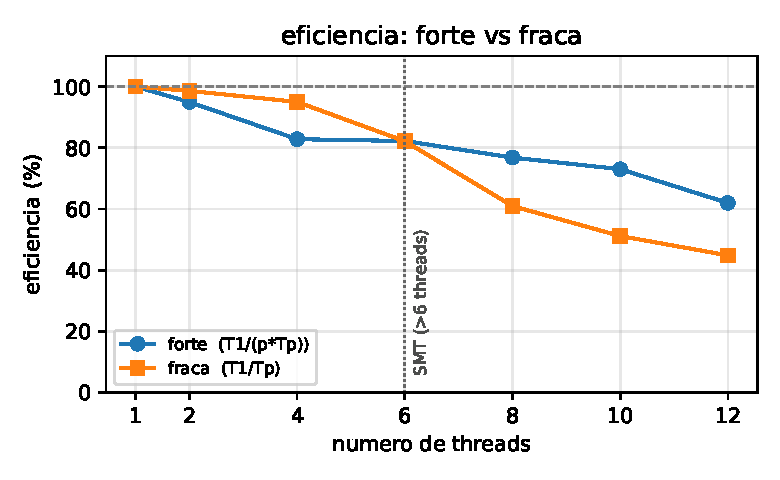
\includegraphics[width=\linewidth]{../results/efficiency.pdf}
  \captionof{figure}{Eficiencia das duas escalabilidades. As duas curvas
    quebram ao entrar no SMT; a partir de 8 threads a fraca cai mais,
    porque cada nucleo passa a receber duas cargas completas.}
  \label{fig:eff}
\end{center}

\section*{7. Uso de ferramentas de IA}
Usamos um assistente de IA para revisar o arnes de medicao, o script de
plotagem e a estrutura do relatorio. Cada decisao de codigo (escopo das
clausulas, escolha de \texttt{dynamic,4}, rng por linha, \texttt{nowait})
foi verificada com as medicoes acima e reproduz-se com o \texttt{README.md}.

\end{multicols}

\begin{center}
  \small
  \captionof{table}{Escalabilidade forte (w=800, h=600, spp=32),
    10 execucoes por ponto. $T_1$ e o binario sequencial compilado
    sem \texttt{-fopenmp}.}
  \label{tab:strong}
  \begin{tabular}{r r r r r r}
    \toprule
    Threads & Med.\ (s) & Min (s) & Max (s) & Speed-up & Ef. \\
    \midrule
    1 ($T_1$) & 53{,}996 & 53{,}552 & 56{,}206 & 1{,}000 & 100{,}0\% \\
    2  & 28{,}437 & 28{,}126 & 30{,}418 & 1{,}899 & 94{,}9\% \\
    4  & 16{,}300 & 15{,}307 & 16{,}929 & 3{,}313 & 82{,}8\% \\
    6  & 10{,}945 & 10{,}512 & 12{,}057 & 4{,}933 & 82{,}2\% \\
    8  &  8{,}789 &  8{,}349 &  9{,}032 & 6{,}144 & 76{,}8\% \\
    10 &  7{,}395 &  6{,}991 &  7{,}672 & 7{,}302 & 73{,}0\% \\
    12 &  7{,}261 &  6{,}456 &  7{,}846 & 7{,}437 & 62{,}0\% \\
    \bottomrule
  \end{tabular}
\end{center}

\begin{center}
  \small
  \captionof{table}{Escalabilidade fraca (w=800, h=600, spp base = 32),
    10 execucoes por ponto. Regra: $\mathrm{spp} = 32 \cdot p$ (custo
    linear em spp; trabalho total escala com $p$). Eficiencia $= T_1/T_p$.}
  \label{tab:weak}
  \begin{tabular}{r r r r r r}
    \toprule
    Threads & spp & Med.\ (s) & Min (s) & Max (s) & Ef. \\
    \midrule
    1 ($T_1$) &  32 & 55{,}643 & 54{,}551 & 57{,}554 & 100{,}0\% \\
    2  &  64 & 56{,}432 & 55{,}605 & 59{,}526 & 98{,}6\% \\
    4  & 128 & 58{,}578 & 57{,}927 & 59{,}572 & 95{,}0\% \\
    6  & 192 & 67{,}730 & 60{,}617 & 73{,}468 & 82{,}2\% \\
    8  & 256 & 91{,}290 & 76{,}362 & 102{,}594 & 61{,}0\% \\
    10 & 320 & 108{,}754 & 107{,}091 & 110{,}528 & 51{,}2\% \\
    12 & 384 & 124{,}098 & 123{,}328 & 125{,}584 & 44{,}8\% \\
    \bottomrule
  \end{tabular}
\end{center}

\begin{center}
  \small
  \captionof{table}{Comparacao de politicas de escalonamento em 12
    threads, 10 execucoes por politica; mesma entrada da escalabilidade
    forte.}
  \label{tab:sched}
  \begin{tabular}{l r r r}
    \toprule
    Politica & Mediana (s) & Min (s) & Max (s) \\
    \midrule
    static               & 9{,}556 & 7{,}573 & 11{,}779 \\
    static, 32           & 8{,}389 & 7{,}425 & 10{,}494 \\
    static, 4            & 7{,}658 & 7{,}259 &  8{,}287 \\
    dynamic              & 7{,}297 & 7{,}210 &  7{,}933 \\
    dynamic, 32          & 7{,}199 & 7{,}157 &  7{,}608 \\
    dynamic, 4 (adotada) & 7{,}164 & 7{,}006 &  7{,}354 \\
    guided               & 7{,}231 & 6{,}935 &  7{,}385 \\
    \bottomrule
  \end{tabular}
\end{center}

\end{document}
